

\tikzset{every picture/.style={line width=0.75pt}} %set default line width to 0.75pt        

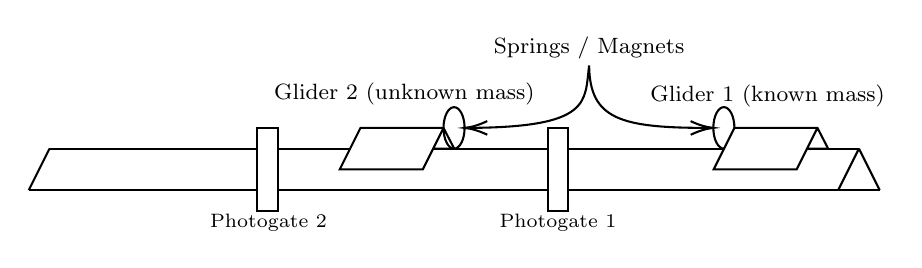
\begin{tikzpicture}[x=0.75pt,y=0.75pt,yscale=-1,xscale=1]
%uncomment if require: \path (0,300); %set diagram left start at 0, and has height of 300

%Straight Lines [id:da5572434639926174] 
\draw    (110,140) -- (520,140) ;


%Straight Lines [id:da02244511382700587] 
\draw    (110,140) -- (120,120) ;


%Straight Lines [id:da5497476983892675] 
\draw    (120,120) -- (510,120) ;


%Straight Lines [id:da57322939128216] 
\draw    (510,120) -- (520,140) ;


%Straight Lines [id:da2970462263374636] 
\draw    (510,120) -- (500,140) ;


%Shape: Rectangle [id:dp04813805212125999] 
\draw  [fill={rgb, 255:red, 255; green, 255; blue, 255 }  ,fill opacity=1 ] (220,110) -- (230,110) -- (230,150) -- (220,150) -- cycle ;
%Shape: Rectangle [id:dp8954323751602662] 
\draw  [fill={rgb, 255:red, 255; green, 255; blue, 255 }  ,fill opacity=1 ] (360,110) -- (370,110) -- (370,150) -- (360,150) -- cycle ;
%Shape: Polygon [id:ds6910058608548333] 
\draw  [fill={rgb, 255:red, 255; green, 255; blue, 255 }  ,fill opacity=1 ] (269.85,110.02) -- (309.85,110.02) -- (315,120) -- (304.85,120.02) -- (309.85,110.02) -- (299.85,130.02) -- (259.85,130.02) -- cycle ;
%Shape: Ellipse [id:dp9683169570061398] 
\draw   (309.85,110.02) .. controls (309.85,104.5) and (312.12,100.02) .. (314.93,100.02) .. controls (317.73,100.02) and (320,104.5) .. (320,110.02) .. controls (320,115.54) and (317.73,120.02) .. (314.93,120.02) .. controls (312.12,120.02) and (309.85,115.54) .. (309.85,110.02) -- cycle ;
%Shape: Ellipse [id:dp16081275394461825] 
\draw   (439.85,110) .. controls (439.85,104.48) and (442.12,100) .. (444.93,100) .. controls (447.73,100) and (450,104.48) .. (450,110) .. controls (450,115.52) and (447.73,120) .. (444.93,120) .. controls (442.12,120) and (439.85,115.52) .. (439.85,110) -- cycle ;
%Curve Lines [id:da5533059977720132] 
\draw    (380,80) .. controls (380.36,105.8) and (394.92,110.07) .. (437.87,110.01) ;
\draw [shift={(439.85,110)}, rotate = 539.75] [color={rgb, 255:red, 0; green, 0; blue, 0 }  ][line width=0.75]    (10.93,-3.29) .. controls (6.95,-1.4) and (3.31,-0.3) .. (0,0) .. controls (3.31,0.3) and (6.95,1.4) .. (10.93,3.29)   ;

%Curve Lines [id:da37032335488484347] 
\draw    (380,80) .. controls (377.74,97.33) and (381.64,109.75) .. (321.83,110.01) ;
\draw [shift={(320,110.02)}, rotate = 359.98] [color={rgb, 255:red, 0; green, 0; blue, 0 }  ][line width=0.75]    (10.93,-3.29) .. controls (6.95,-1.4) and (3.31,-0.3) .. (0,0) .. controls (3.31,0.3) and (6.95,1.4) .. (10.93,3.29)   ;

%Shape: Polygon [id:ds012853840364027702] 
\draw  [fill={rgb, 255:red, 255; green, 255; blue, 255 }  ,fill opacity=1 ] (450,110) -- (490,110) -- (495.15,119.98) -- (485,120) -- (490,110) -- (480,130) -- (440,130) -- cycle ;

% Text Node
\draw (365,155.5) node  [font=\footnotesize] [align=left] {{\scriptsize Photogate 1}};
% Text Node
\draw (225.5,155.5) node  [font=\footnotesize] [align=left] {{\scriptsize Photogate 2}};
% Text Node
\draw (291,93.5) node  [font=\scriptsize] [align=left] {{\footnotesize Glider 2 (unknown mass)}};
% Text Node
\draw (466,94.5) node  [font=\scriptsize] [align=left] {{\footnotesize Glider 1 (known mass)}};
% Text Node
\draw (380,71.5) node  [font=\footnotesize] [align=left] {Springs / Magnets};


\end{tikzpicture}
